\chapter{Implementierung}
\label{ch:implementierung}

In diesem Kapitel werden die Vorgehensweisen und Verwendungen der Technologien beschrieben. Hierbei wird zuerst auf die Ladestation eingegangen, da dort die Funktionsweise der peripheren Geräte erklärt wird, die für die Implementierung der Server-Logik wichtig sind. Anschließend folgt der Server und zum Schluss die Steuercontroller. \\
Der Quellcode des Projekts ist unter der Referenz \cite{PROJEKT} zu finden.


\section{Das Tor}
Das Tor an sich beinhaltet keine Funktionalität, außer ein Ziel für die Spieler darzustellen. Die eigentlichen Funktionen befinden sich in den folgenden Komponenten, die in das Tor integriert wurden.


\subsection{Infrarot-LED}
\label{sec:infrarot_led}
Die Infrarot-LED dient dazu, dem Roboter die Richtung zu vermitteln, in der seine Ladestation, also sein Tor zu finden ist. Bei dieser Art der Kommunikation gibt es nur einen Sender und einen Empfänger. Die Infrarot-LED nimmt hierbei die Rolle des Senders ein und der Roboter die des Empfängers. 
Um die Funktionalität der Kommunikation besser zu vermitteln, wird im Folgenden zunächst auf die technischen Grundlagen bei der IR-Kommunikation eingegangen.
Der Infrarot Empfänger besteht aus einer Photodiode, einem bei einer gewissen Frequenz geregeltem Verstärker und einem Demodulator. Bei unserem Empfänger beträgt die Verstärkerfrequenz etwa 38 kHz. Nun ist es möglich, Signale mit der IR-LED zu erzeugen, die dann vom Empfänger verarbeitet werden. Hierbei beträgt die Trägerfrequenz des modulierten Signals genau die Frequenz, auf der der Verstärker des Empfängers arbeitet, also 38 kHz. Das Signal besteht aus zwei Werten, entweder aus der 0, also die IR-LED ist aus, oder aus einer logischen 1, indem die IR-LED mit diesen 38 kHz blinkt. Gemessen werden kann nun die Frequenz, die aus der Dauer der logischen 1 und der logischen 0 resultiert. 

Realisiert wurde diese Frequenz mit dem Timerbaustein NE555, an den die drei LEDs parallel zueinander geschaltet sind. Diese lassen sich mithilfe von Transistoren vom RaspberryPi aus unterschiedlich lang an und ausschalten. Der Schaltplan inklusive Bauteilwerte befindet sich im Anhang \ref{fig:schaltplan_ne555}

\begin{figure}[!h]
	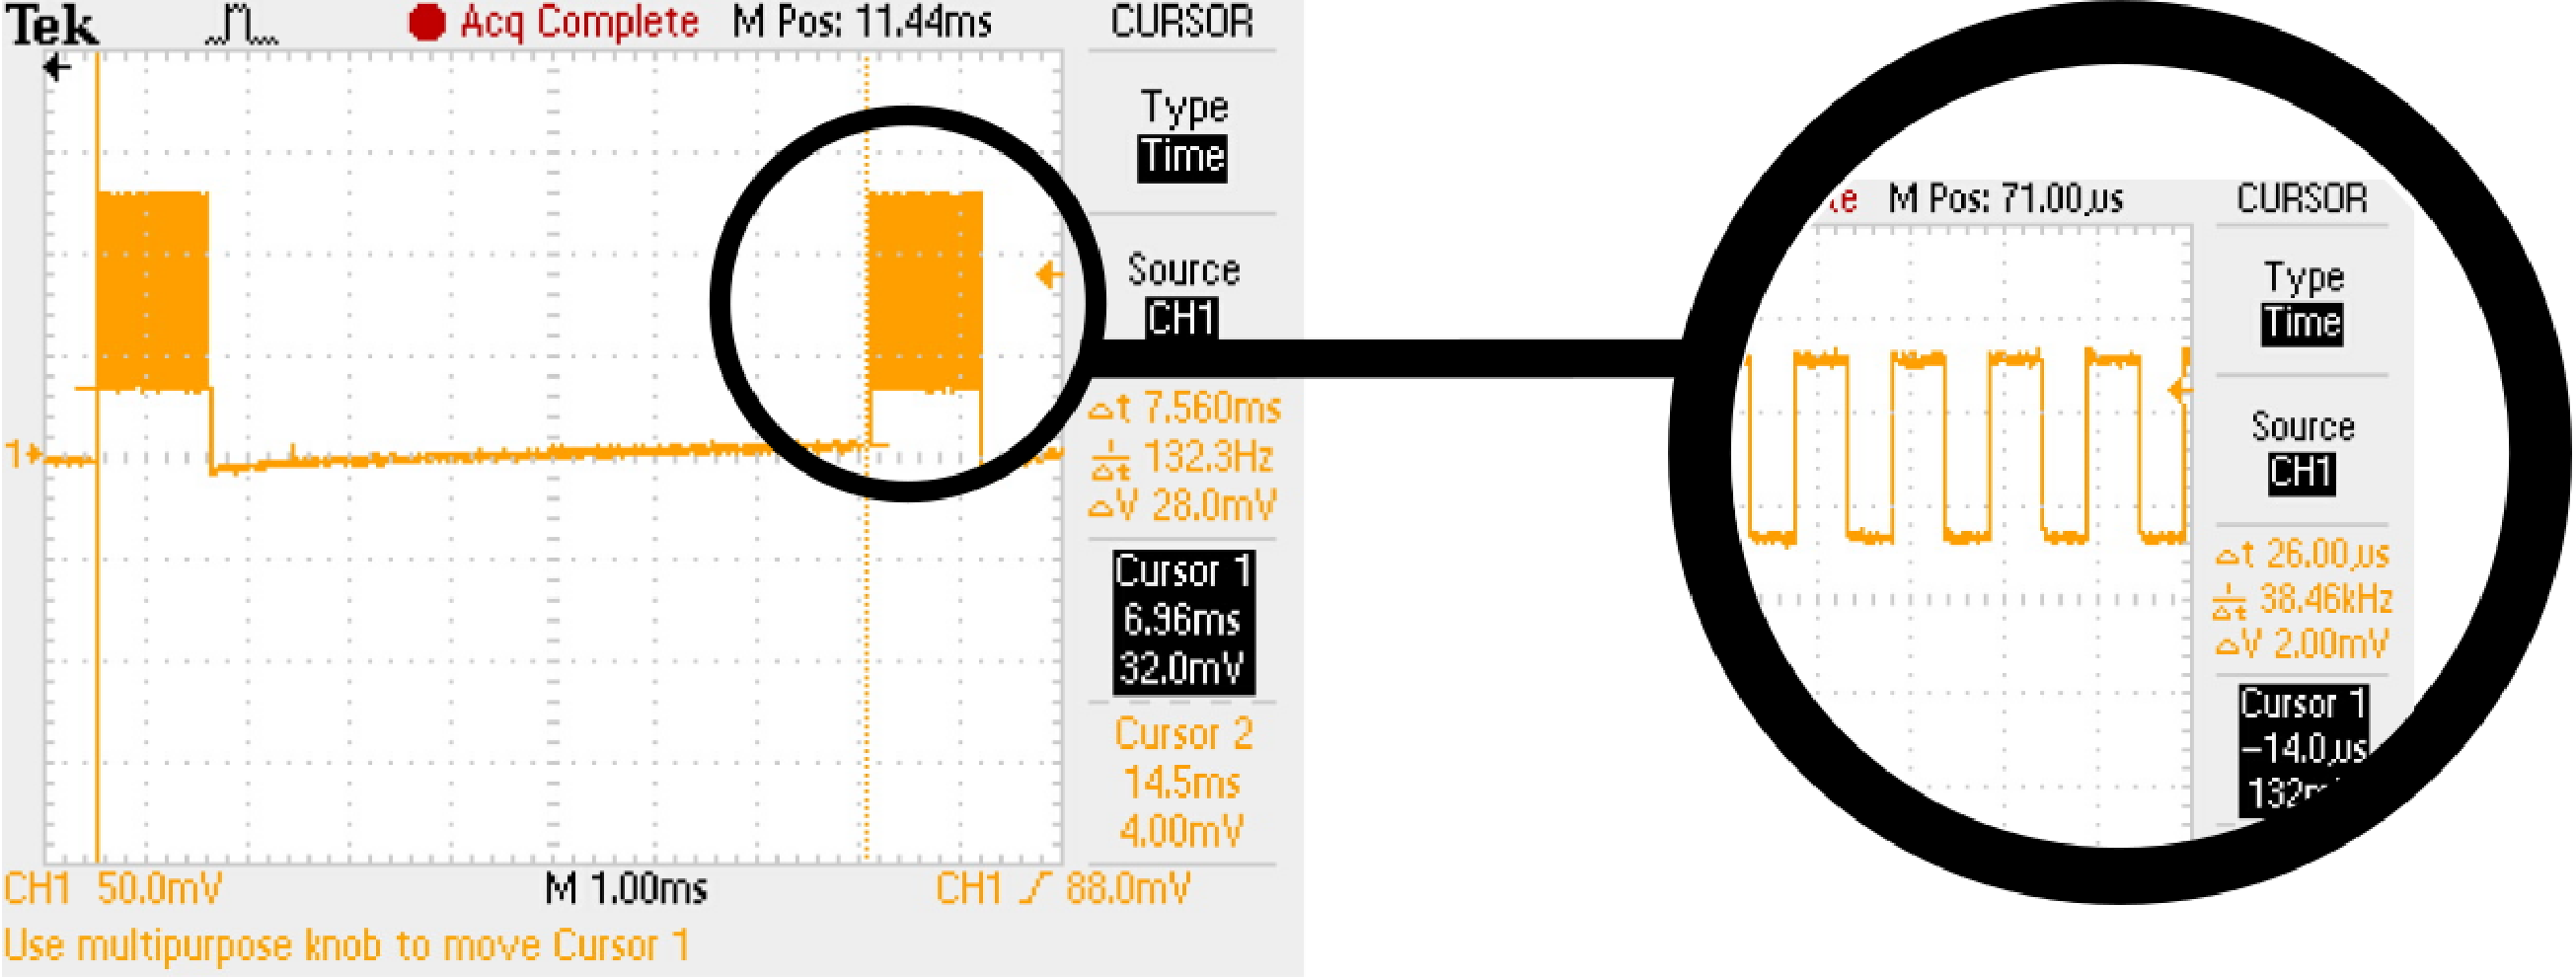
\includegraphics[width=\textwidth]{images/ir_burst_with_zoom.pdf}
	\caption{Beispiel Burst mit einer postivien Pulslänge von ca. 1ms und ca. 6,4ms Pause}
	\label{fig:ir_burst}
\end{figure}

\begin{figure}[!h]
	\centering
	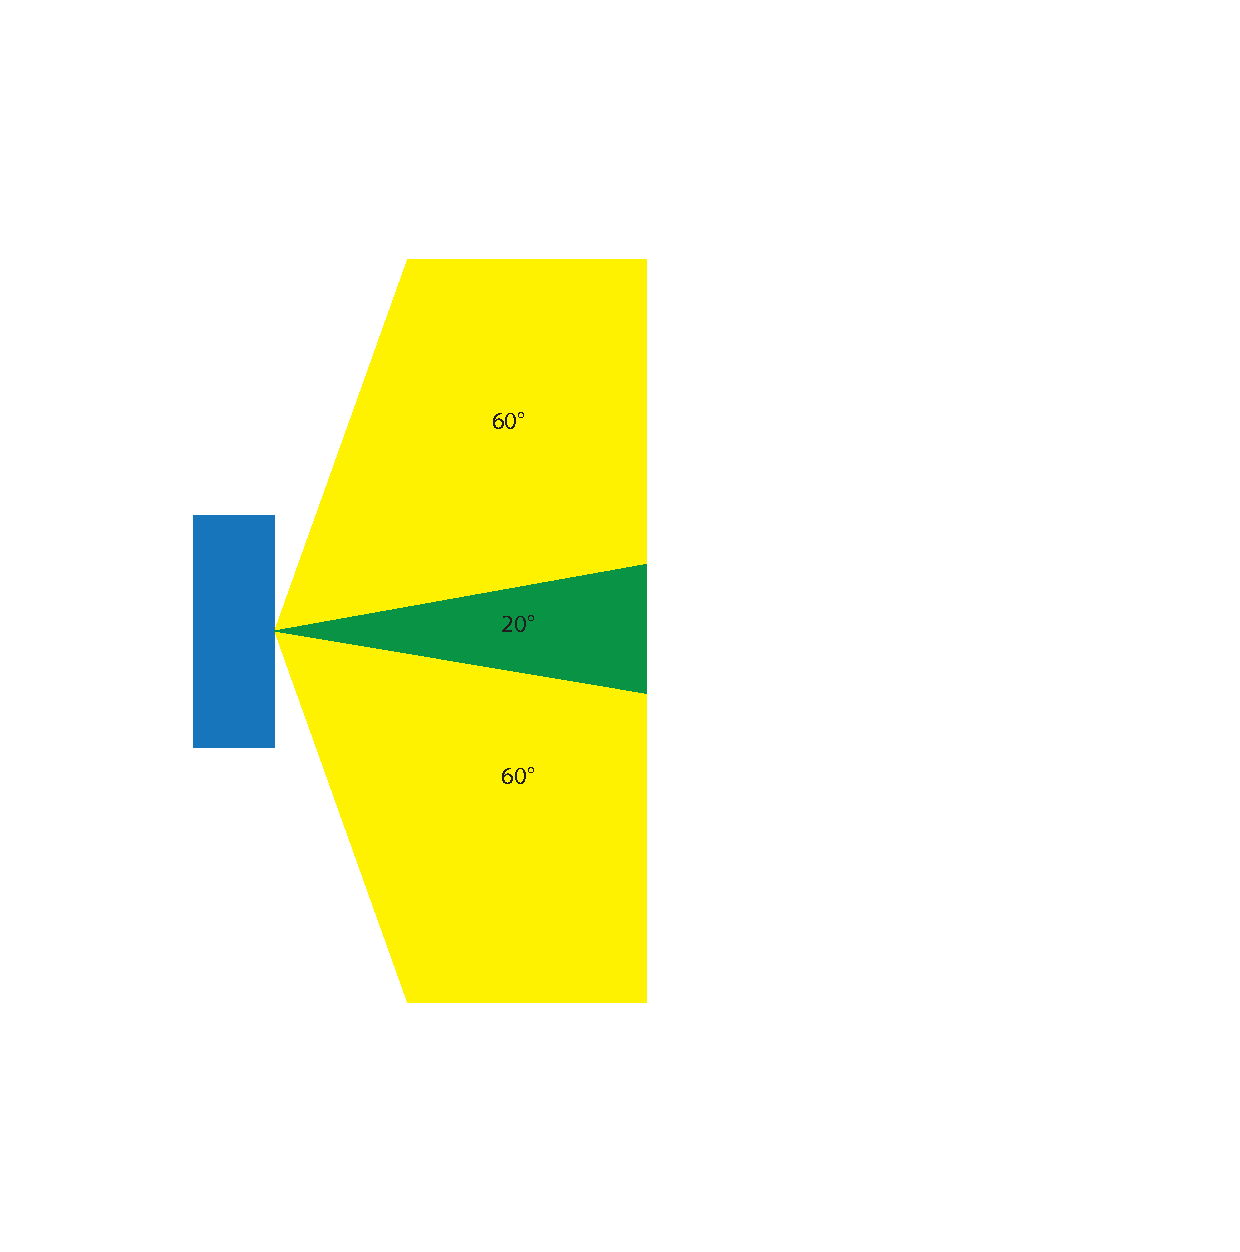
\includegraphics[width=\textwidth]{images/ir_led_aufbau.pdf}
	\caption{Schematischer Aufbau der Infrarot LED mit Abstrahlwinkel}
	\label{fig:ir_led_aufbau}
\end{figure}

Der Aufbau ist wie in Abbildung \ref{fig:ir_led_aufbau} zu sehen folgendermaßen:
Am oberen Endes Tores sind drei Infrarot-LEDs befestigt. Die äußeren beiden haben einen Abstrahlwinkel von 40\degree  und die mittlere einen von 20\degree. Diese sind so angeordnet, dass sich die Signale nicht überschneiden. Auf dem Roboter ist der Empfänger auf derselben Seite wie die Ladekontakte platziert. Hierbei muss beachtet werden, dass der Empfänger seitlich abgeschirmt ist, das bedeutet er bekommt nur Signale die tatsächlich frontal auf ihn eintreffen.

Um den Ladeprozess möglichst fehlerfrei zu starten ist es notwendig, dass der Roboter möglichst frontal auf die Ladestation zu fährt, deshalb hat die mittlere LED nur einen Abstrahlwinkel von 20\degree  (maximal 10\degree  Abweichung). Diese ist somit die LED, die signalisiert, dass der Roboter nun korrekt platziert ist und sich nur noch gerade aus auf die LED zu bewegen muss. Die anderen beiden LEDs dienen dem Zweck, den Roboter in genau diese Position zu bringen. Da die LEDs unterschiedlich moduliert sind, kann der Roboter erkennen in welchem Signal er sich nun befindet. Ist es die mittlere, fährt er gerade aus auf das Tor, ist es eine der äußeren, bewegt er sich weiter zur Mitte. (vgl. Abschnitt \ref{sec:torfindung})


\subsection{Ladestation}
Die Kontakte der Ladestation wurden mithilfe einfacher Kupferstreifen realisiert, die am Tor angebracht wurden. Diese sind direkt mit einem Ladegerät verbunden. (Näheres hierzu in Referenz \cite{ALEX})

\subsection{Torerkennung}
Für die Torerkennung waren mehrere Technologien denkbar. Möglichkeit 1 wäre gewesen das Tor mit einer Lichtschranke zu versehen. Möglichkeit 2 wäre die Entwicklung eines intelligenten Balls, der selbstständig erkennt ob er sich im Tor befindet und Möglichkeit 3 wäre die Konstruktion eines simplen Tasters, der durch den eintreffenden Ball betätigt wird.
Möglichkeit 2 wurde schon zu Beginn verworfen, da der Ball selbst eine Komponente darstellen würde und deshalb nicht leicht austauschbar wäre und vor allem ebenfalls mit Strom versorgt werden müsste, was wieder eine Ladestation erfordert. Man müsste ihn so konzipieren, dass er durch die auf ihn einwirkenden Kräfte nicht zerstört würde, da sobald er mal nicht mehr funktionsfähig wäre, man nicht mehr spielen könnte bis ein neuer Ball gefertigt wurde. \\
Das Problem bei Möglichkeit 1 und 3 ist folgendes: Beide erkennen lediglich eine Bewegung im Tor, es kann aber nicht sichergestellt werden, ob die Bewegung tatsächlich von dem Ball aus geht. So ist es deshalb möglich, einfach mit dem Roboter an das Tor zu fahren und zu hoffen, dass der Roboter weit genug in das Tor hinein ragt. Die Entscheidung fiel schließlich auf die Variante mit dem mechanischen Taster. Im Gegensatz zu der Lichtschranke, ist dieser nicht anfällig gegen andere Lichteinwirkungen, die nur mit erheblichem Mehraufwand gefiltert werden könnten. \\
Der mechanische Schalter ist eine simple \glqq Klappenkonstruktion\grqq. Im Tor befindet sich eine Messingstange an der eine Klappe hängt. An der Rückseite dieser Klappe befinden sich Kupferstreifen, die, sobald ein Ball die Klappe nach hinten drückt, eine Verbindung zwischen zwei Kontakten herstellen. Das bewirkt eine Zustandsänderung auf einem GPIO-Pin des RaspberryPi's, die vom Server erkannt wird.

\section{Server}
\label{impl:server}
Der Server hat die Aufgabe, die gesamte Kommunikation zwischen Controllern und Robotern zentral zu verwalten und zu koordinieren. Auch die Spiellogik und Interpretation der Steuerbefehle ist Aufgabe des Servers. Außerdem müssen die Eingabe und Ausgabe der Peripheriegeräte verwaltet, bzw. gesteuert werden. Diese Peripheriegeräte sind die Ladestation, die gefunden werden muss, die Torerkennung, die verarbeitet werden muss und die Infrarot-LED, mithilfe der die Ladestation gefunden werden kann. Die Bilddaten, die vom Roboter versendet werden, müssen hier zwischengespeichert werden und anschließend an die Controller weiter gegeben werden.

\subsection{Verbindung}
Die Verbindungslogik besteht im Wesentlichen aus fünf Klassen, die in Abbildung \ref{fig:uml_verbindung} dargestellt sind. Verwaltet werden die Verbindungen in der Klasse \textit{ConnectionManager}, der die Verbindungen für die Spiellogik bereit stellt, sobald ein Controller-Roboter paar verbunden wurde. Für die Verbindungen der Controller gibt es \textit{WebsocketSocket}. Ein Objekt dieser Klasse dient als Schnittstelle der Kommunikation zwischen einem Controller und dem Server. Hierbei werden die Nachrichten im JSON-Format ausgetauscht, da dies eine Key-Value Kommunikation ermöglicht und für abstrakte Sprachen wie Javascript leichter zu verwenden ist als eine Byte-Orientierte Übertragung. Aufgerufen wird die Schnittstelle über die URL: \url{ws://ip\_des\_servers:8080/control/}. Für die Verbindungen der Roboter gibt es \textit{UDPConnectionHandler}. Auch ein Objekt davon steht für genau eine Verbindung mit einem Roboter, jedoch werden die Befehle hier im Gegensatz zu den WebSockets Byte-Orientiert ausgetauscht. Um eine Verbindung mit einem Roboter herzustellen, wird in der Klasse \textit{UDPSocketProvider} auf Port 44044 auf eingehende Pakete gewartet und anschließend ein Socket zu diesem Endpunkt bereit gestellt. Diese Klasse implementiert das \textit{Runnable} Interface und wird als eigener Thread gestartet \cite{PROJEKT}.  Auch die Authentifizierung wird in dieser Klasse abgehandelt, indem überprüft wird, ob die eingehenden Pakete einer der IP-Adressen der Roboter zugeordnet werden können. Da die Roboter statische IP-Adressen bekommen sollen ist diese Methode überhaupt möglich. Zusätzlich gibt es für den \textit{UDPConnectionHandler} eine Hilfsklasse, die \textit{ConnectionControl}. In dieser wird festgelegt, wie lange die Verbindung als offen gekennzeichnet werden soll, obwohl kein Paket ankommt. Auf der Controllerseite wird eine solche Implementierung nicht benötigt, da der WebSocket auf HTTP und damit auf TCP basiert. Ein Verbindungsabbruch ist dort auch ohne Timeout erkennbar.


\begin{figure}[!h]
	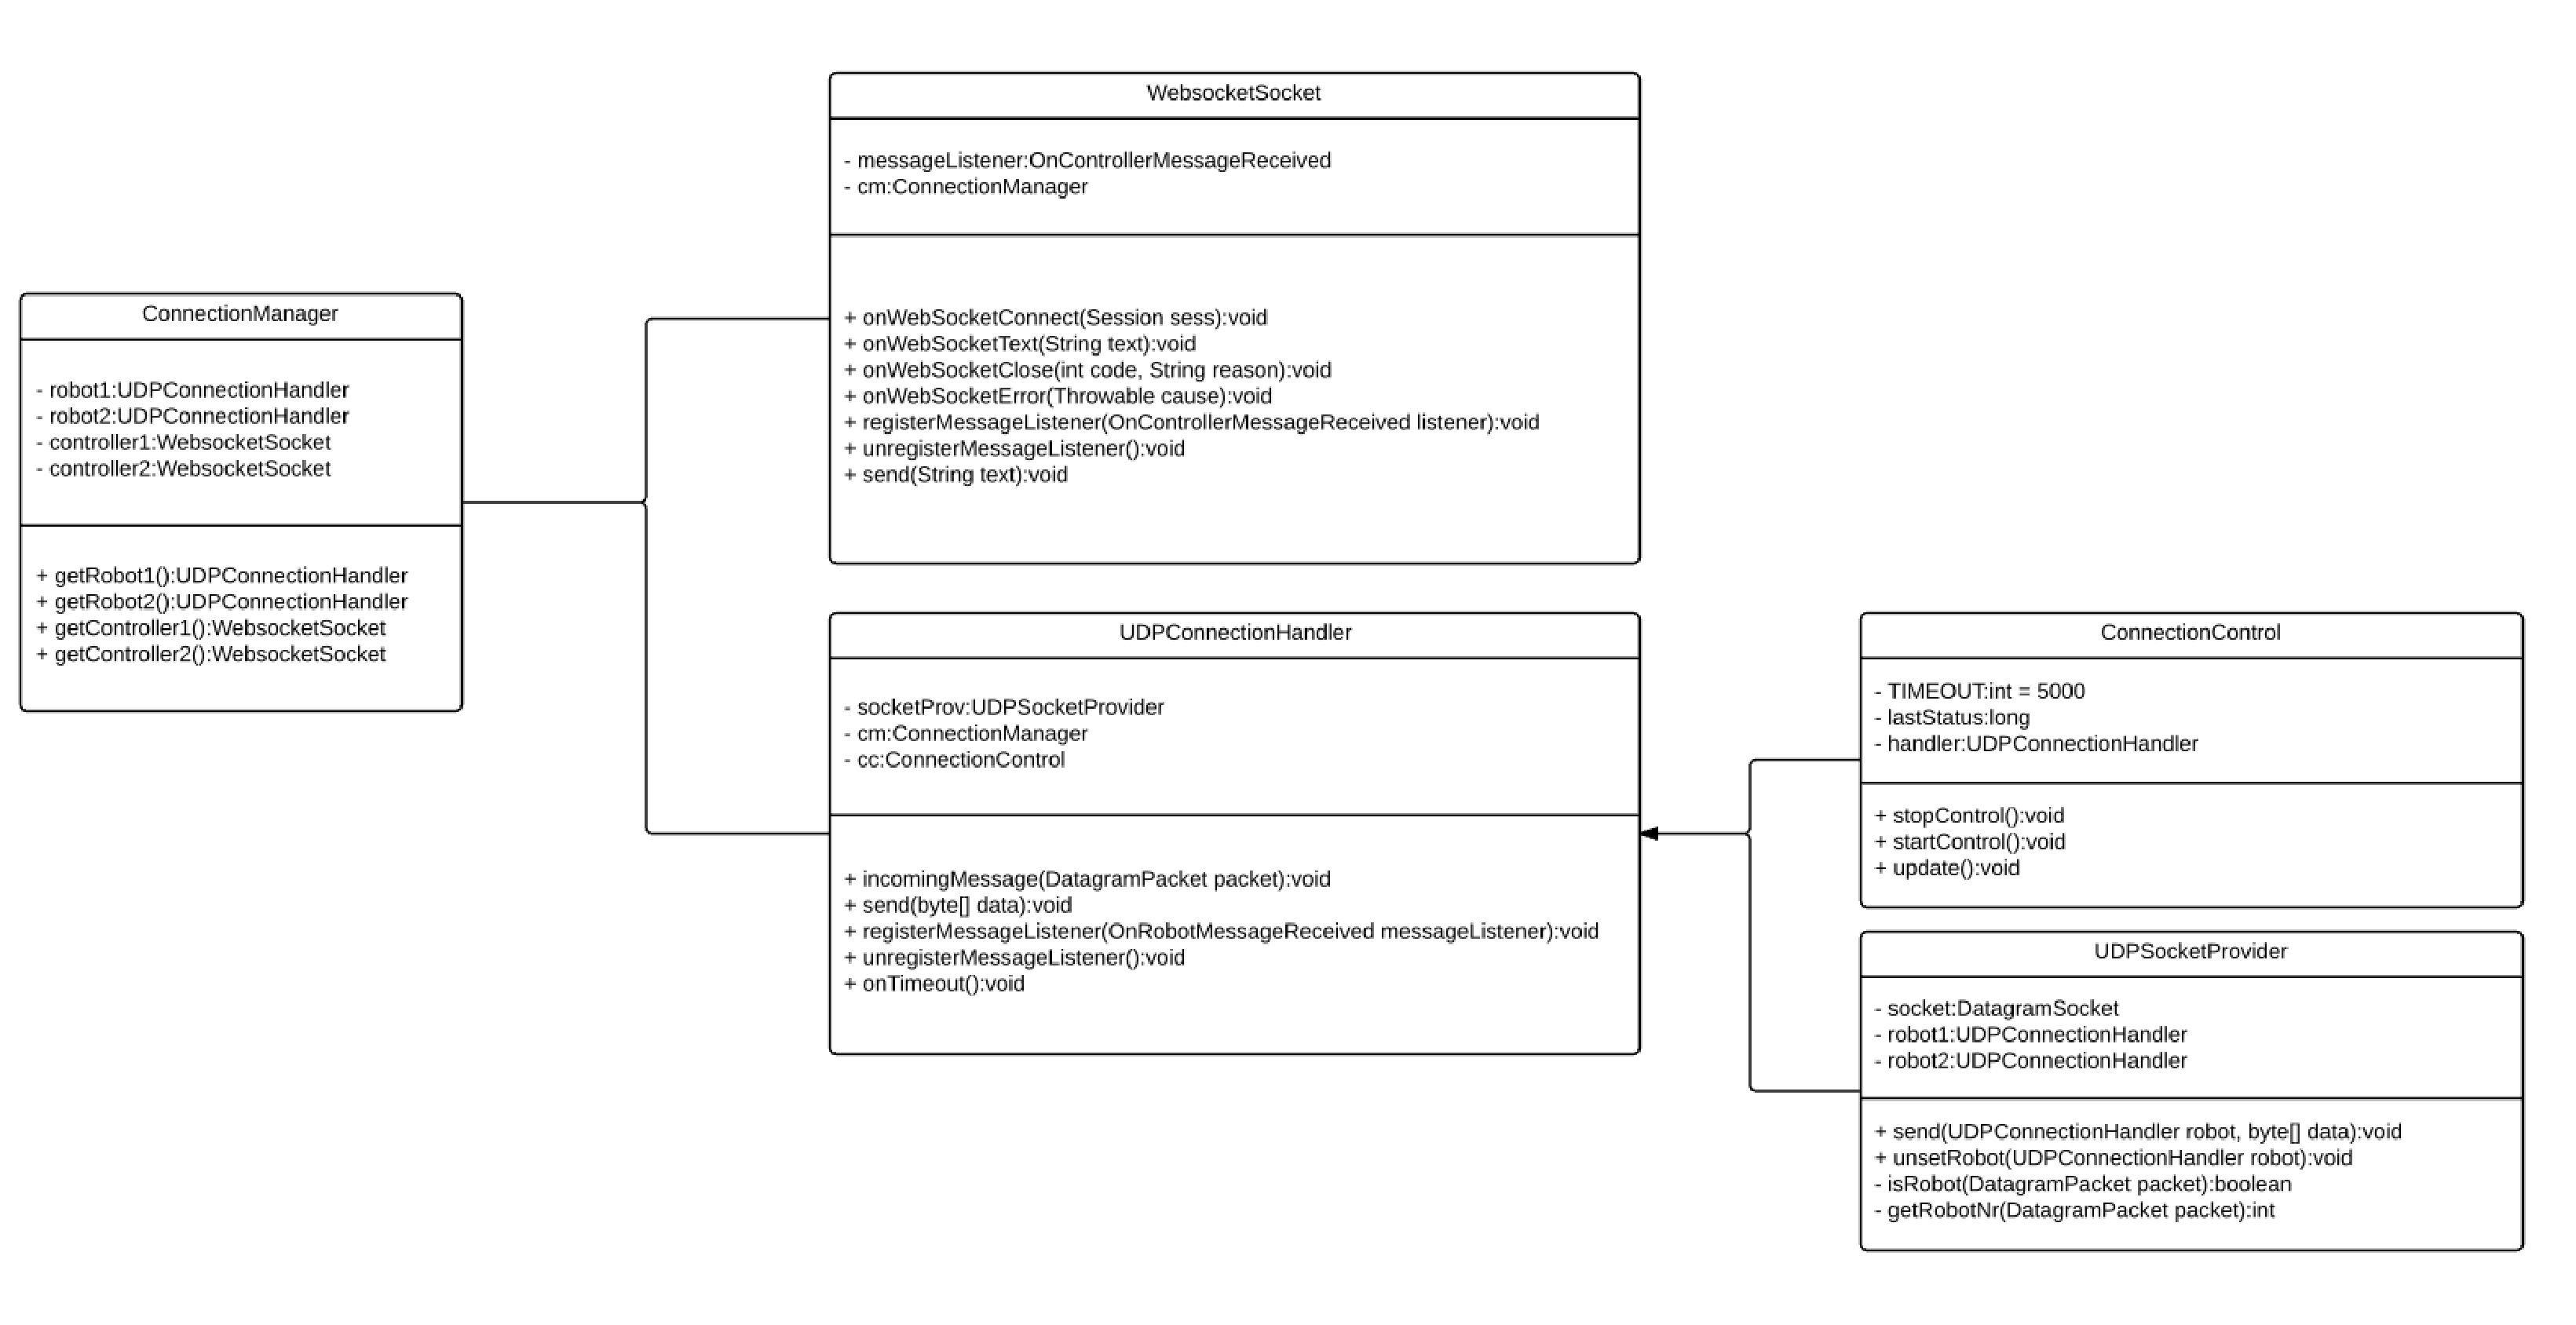
\includegraphics[width=\textwidth]{images/uml_verbindung.pdf}
	\caption{Klassendiagramm der Verbindungslogik}
	\label{fig:uml_verbindung}
\end{figure}



\subsection{Steueralgorithmen}
Da die verschiedenen Steuervarianten unterschiedliche Steuerparameter erzeugen ist es für jede einzelne davon notwendig, diese zu interpretieren und in eine Form zu bringen, die mit der Schnittstelle zum Roboter kompatibel ist. Auf diese wird in den nächsten Abschnitten genauer eingegangen. Das heißt, am Ende der Übersetzung müssen die Geschwindigkeiten der Motoren links und rechts und ob ein Schuss ausgelöst werden soll. Unabhängig der Steuervariante muss der Ausgangsbefehl anhand des vorherigen Befehls nachkorrigiert werden. Da die Motoren des Roboters eine im Vergleich zur Haftreibung der Räder hohe Beschleunigung aufweisen, müssen die Beschleunigungen begrenzt werden, um durchdrehende Räder und damit ein unkontrollierbares Verhalten der Steuerung zu vermeiden. 
Dies wird realisiert, indem ein maximal möglicher folgender Motorwert anhand des vorhergehenden Motorwertes errechnet wird. Die Berechnungsformel ist relativ simpel, der neue Wert darf um maximal einen festen Wert x größer sein als der alte Wert. Das ist dadurch zu begründen, dass für die Überschreitung der Haftreibung der Räder lediglich die dort wirkende Kraft ausschlaggebend ist, die wiederum aus der Beschleunigung der Räder resultiert. Dieser Wert x wurde nach einigen Testversuchen auf 10 festgelegt. Für den Fall, das beide gewünschten Motorenwerte über dem errechneten erlaubten Maximum liegen, muss anschließend das Verhältnis von linkem zu rechtem Motor angepasst werden, da sonst beide werte gleichgestellt werden, auch wenn diese sich zuvor unterschieden hätten. 
Zur Veranschaulichung dieser Korrektur ist in Tabelle \ref{tab:bsp_korrektur} ein Beispiel aufgeführt. Wie man sieht wünscht der Benutzer durch seine Eingabe einen leichten Bogen nach rechts zu fahren, jedoch würden nach der Maximalwertkorrektur beide Motoren gleich schnell bewegt werden. Erst nach der Anpassung des Verhältnisses fährt der Roboter tatsächlich den gewünschten Radius.

\vspace{1cm}

\begin{table}[h!]
	\begin{tabularx}{\textwidth}{|X|X|X|X|X|}
		\hline
		 & letzte Motorbefehle & neue Motorbefehle & nach Korrektur (ohne Verhältnis) & nach Korrektur (mit Verhältnis) \\ \hline
		Motor Links      & 50      & 80      & 60      &
		06  \\
		Motor Rechts      & 50      & 70      & 60
		& 52 \\ \hline
	\end{tabularx}
	\caption{Motor Werte nach Durchlaufen des Korrekturalgorithmus}
	\label{tab:bsp_korrektur}
\end{table}



\subsubsection{Differential Steuerung}
Da die eingehenden Steuerparameter direkt die Motorenbefehle für Links und Rechts beinhalten (vgl. Abschnitt \ref{sec:differentialsteuerung}), ist hier keine weitere Interpretation notwendig. 

\subsubsection{RC-Remote Steuerung}
\label{sec:rcremote_server}
Die eingehenden Steuerparameter sind der Vorschub und die Richtung. Der Vorschub lässt sich direkt auf die Motoren übertragen, lediglich die Richtung muss mittels einer Formel berechnet werden. Der Interval indem sich der Wert der Richtung befindet ist [-50, 50]. An dieser Stelle bietet sich eine Exponentialformel an. 
Im Allgemeinen lautet diese: 
{\Large \[ratio_{LR} = a^{\frac{x}{50}}\]},
wobei der Parameter a bestimmt, wie groß das Verhältnis bei maximaler Auslenkung ist und x den momentanen Richtungswert angibt.
Nach einigen Testläufen wurde der Parameter a zu 2 bestimmt. Dadurch bewegt sich der linke Motor mindestens halb so schnell und maximal doppelt so schnell wie der rechte Motor. Der zugehörige Code ist in Listing \ref{code:rc_motor} zu sehen.

\begin{lstlisting}[captionpos = b, caption=Umrechnung der RC Parameter in Motorbefehle, label = code:rc_motor]
double ratioLR = Math.pow(2,((double) dir/50));
if (ratioLR > 1) {
	robot.setMotorRight(
		(int) ((double) robot.getMotorLeft() / ratioLR)
	); 
}
if (ratioLR < 1) {
	robot.setMotorLeft(
		(int) ((double) robot.getMotorRight() * ratioLR)
	);
}
\end{lstlisting}


\subsubsection{Pfeiltasten Steuerung}
\label{sec:webanwendung_server}
Diese Steuervariante hat einen bedeutenden Nachteil. Da die Eingangsparameter die momentan gedrückten Tasten sind (siehe Abschnitt \ref{sec:webanwendung_anwendung}), gibt es keine Zwischenwerte für die Beschleunigung oder Richtung. Die Taste nach vorne bedeutet hierbei einen Motorschub für beide Seiten von 100\%. Für jede zusätzliche Richtungstaste, also links oder rechts, werden auf der dementsprechenden Seite 25\% abgezogen. Wird nur eine Richtungstaste ohne eine Beschleunigungstaste gedrückt, werden die Motoren auf -15\%/15\% bzw. 15\%/-15\% gesetzt, was einer Drehung auf der Stelle entspricht. Diese \glqq Alles oder Nichts\grqq Steuerung führt im Spiel zu einer nicht flüssigen, jedoch durch die Möglichkeit der Drehung auf der Stelle zu einer annehmbaren Steuerung. Der Code dafür ist in Listing \ref{code:wasd_motor} gezeigt.

\begin{lstlisting}[captionpos = b, caption=Umrechnung der Pfeiltasten in Motorbefehle, label = code:wasd_motor]
if (JSONUtil.jsonObjToBoolean(command.get("up"))) {
	motorLeft += 100;
	motorRight += 100;
}
if (JSONUtil.jsonObjToBoolean(command.get("down"))) {
	motorLeft -= 100;
	motorRight -= 100;
}
if (JSONUtil.jsonObjToBoolean(command.get("right"))) {
	motorRight *= 0.75;
}
if (JSONUtil.jsonObjToBoolean(command.get("left"))) {
	motorLeft *= 0.75;
} 

if (motorRight == 0 && motorLeft == 0 &&
JSONUtil.jsonObjToBoolean(command.get("right"))) {

	motorLeft = 20;
	motorRight = -20;
}

if (motorRight == 0 && motorLeft == 0 &&
JSONUtil.jsonObjToBoolean(command.get("left"))) {

	motorLeft = -20;
	motorRight = 20;
}
\end{lstlisting}
 

\subsection{Bildübertragung}
Wie in der Schnittstellenbeschreibung in Kapitel \ref{sec:schnittstelle} beschrieben, werden die Bilddaten vom Roboter an die Statusnachrichten angehängt. Hierbei kennzeichnen die Bytes FF D8 den Beginn eines neuen Frames. Diese Kombination tritt in JPEG-kodierten Bildern immer nur am Anfang des Bildes auf, wodurch es möglich ist, Bilddaten über mehrere Pakete zu verteilen. Diese Daten werden in der \textit{Player}-Klasse gepuffert, bis das Bild vollständig ist. Anschließend wird es noch base64 kodiert und sofort an die Controller weiter gesendet und nicht mit den regelmäßigen Statusbefehlen, um keine unnötige Zeitverzögerung einzubauen. Die base64 Kodierung wurde im Gegensatz zur einfachen Byte-Orientierten übertragen bevorzugt, damit mit den Controllern in einer höheren Datenabstraktionsebene kommuniziert werden kann. Das vereinfacht den Code vor allem in der Webanwendung, da diese in Javascript implementiert ist. Ein großer Nachteil dieser Kodierung ist der größere Speicherbedarf, der die Übertragung aufgrund höheren Traffics langsamer macht und dadurch zu Verzögerungen führt, die letztendlich im Verlust der Steuerbarkeit resultieren können. Nach ersten Tests ist die Bildrate vom Roboter jedoch so gering, dass diese wenigen Frames rechtzeitig übertragen werden können. Zusätzlich sind die Frames in einer Größenordnung, in der 33 \% Mehrbedarf noch zu keiner Netzwerküberlastung führen.\\ Der Servercode für die Pufferung der Bilddaten des Roboters ist in Listing \ref{code:puffer_pic} aufgeführt.

\begin{lstlisting}[captionpos = b, caption=Logik für die Pufferung der Bilddaten, label = code:puffer_pic]
private void handlePictureData(byte[] data) {
	for (int i = 0; i < data.length; i++) {
		if (data[i] == (byte) 0xFF && 
			i < data.length -1 && 
			data[i+1] == (byte) 0xD8 && 
			pictureBuf.size() != 0) {
			
			sendPicture();
			pictureBuf.reset();
		}
		pictureBuf.write(data[i]);
	}
}
\end{lstlisting}



\subsection{Torfindung}
\label{sec:torfindung}
Mit der Torfindung ist der Vorgang gemeint, um die Ladestation, die im Tor integriert ist zu finden und selbstständig anzufahren. Über die Statusmeldungen des Roboters erfährt der Server wie hoch der Akkustand des Roboters ist. Sobald der Roboter ein Minimum des Akkustands unterschreitet, greift die Torfindung ein. Diese wird in der Klasse \textit{EnergyManager} implementiert (siehe Abb. \ref{fig:uml_energymanager}). Dabei wird die Torfindung sofort aktiviert, wenn sich ein Roboter mit dem Server verbindet und nicht erst wenn noch ein Controller hinzu kommt. Tritt der Fall ein, dass der Akku den Schwellenwert unterschreitet, werden die Infrarot-LEDs über die Klasse \textit{BlinkTask} angeschaltet. Über das \glqq seeGoal\grqq Flag (vgl. Schnittstellenbeschreibung, Kapitel \ref{sec:schnittstelle}) kann erkannt werden, ob das zum Roboter gehörende Tor in Sicht ist oder ob sich der Roboter neben der zum Tor führenden LED befindet. Bekommt der Server vom Roboter drei aufeinander folgende Stati, in denen der Roboter meldet, dass eine LED in Sicht ist, dann fährt der Roboter in die dementsprechende Richtung. Ist der Roboter vom eigenen Tor abgewandt, beginnt sich der Roboter zu drehen, solange bis entweder mindestens ein Status mit positiver Rückmeldung kommt, oder bis ein Timeout abgelaufen ist. Um die Drehung zu unterbrechen genügt deswegen bereits ein Status mit einer Sichtung, um die Möglichkeit einer korrekten Sichtung nicht durch zu schnelles drehen sofort zu verwerfen. Der Timeout bewirkt, dass sich der Roboter nicht endlos um sich selbst dreht, falls er außerhalb des Abstrahlwinkels der LEDs ist. Tritt ein Timeout auf, fährt der Roboter wenige Sekunden in die aktuelle Richtung, um seine Ausgangsposition zufällig zu ändern. Nach diesem Prinzip wird früher oder später eine LED erkannt und das Tor und damit die Ladestation kann angefahren werden. \\ Umgesetzt wurde die Torfindung mithilfe eines Zustandsautomaten (Abbildung \ref{fig:state_findgoal}). Da der Code einige Zeilen umfasst wird an dieser Stelle auf das Projekt verwiesen \cite{PROJEKT}.

\begin{figure}[!h]
	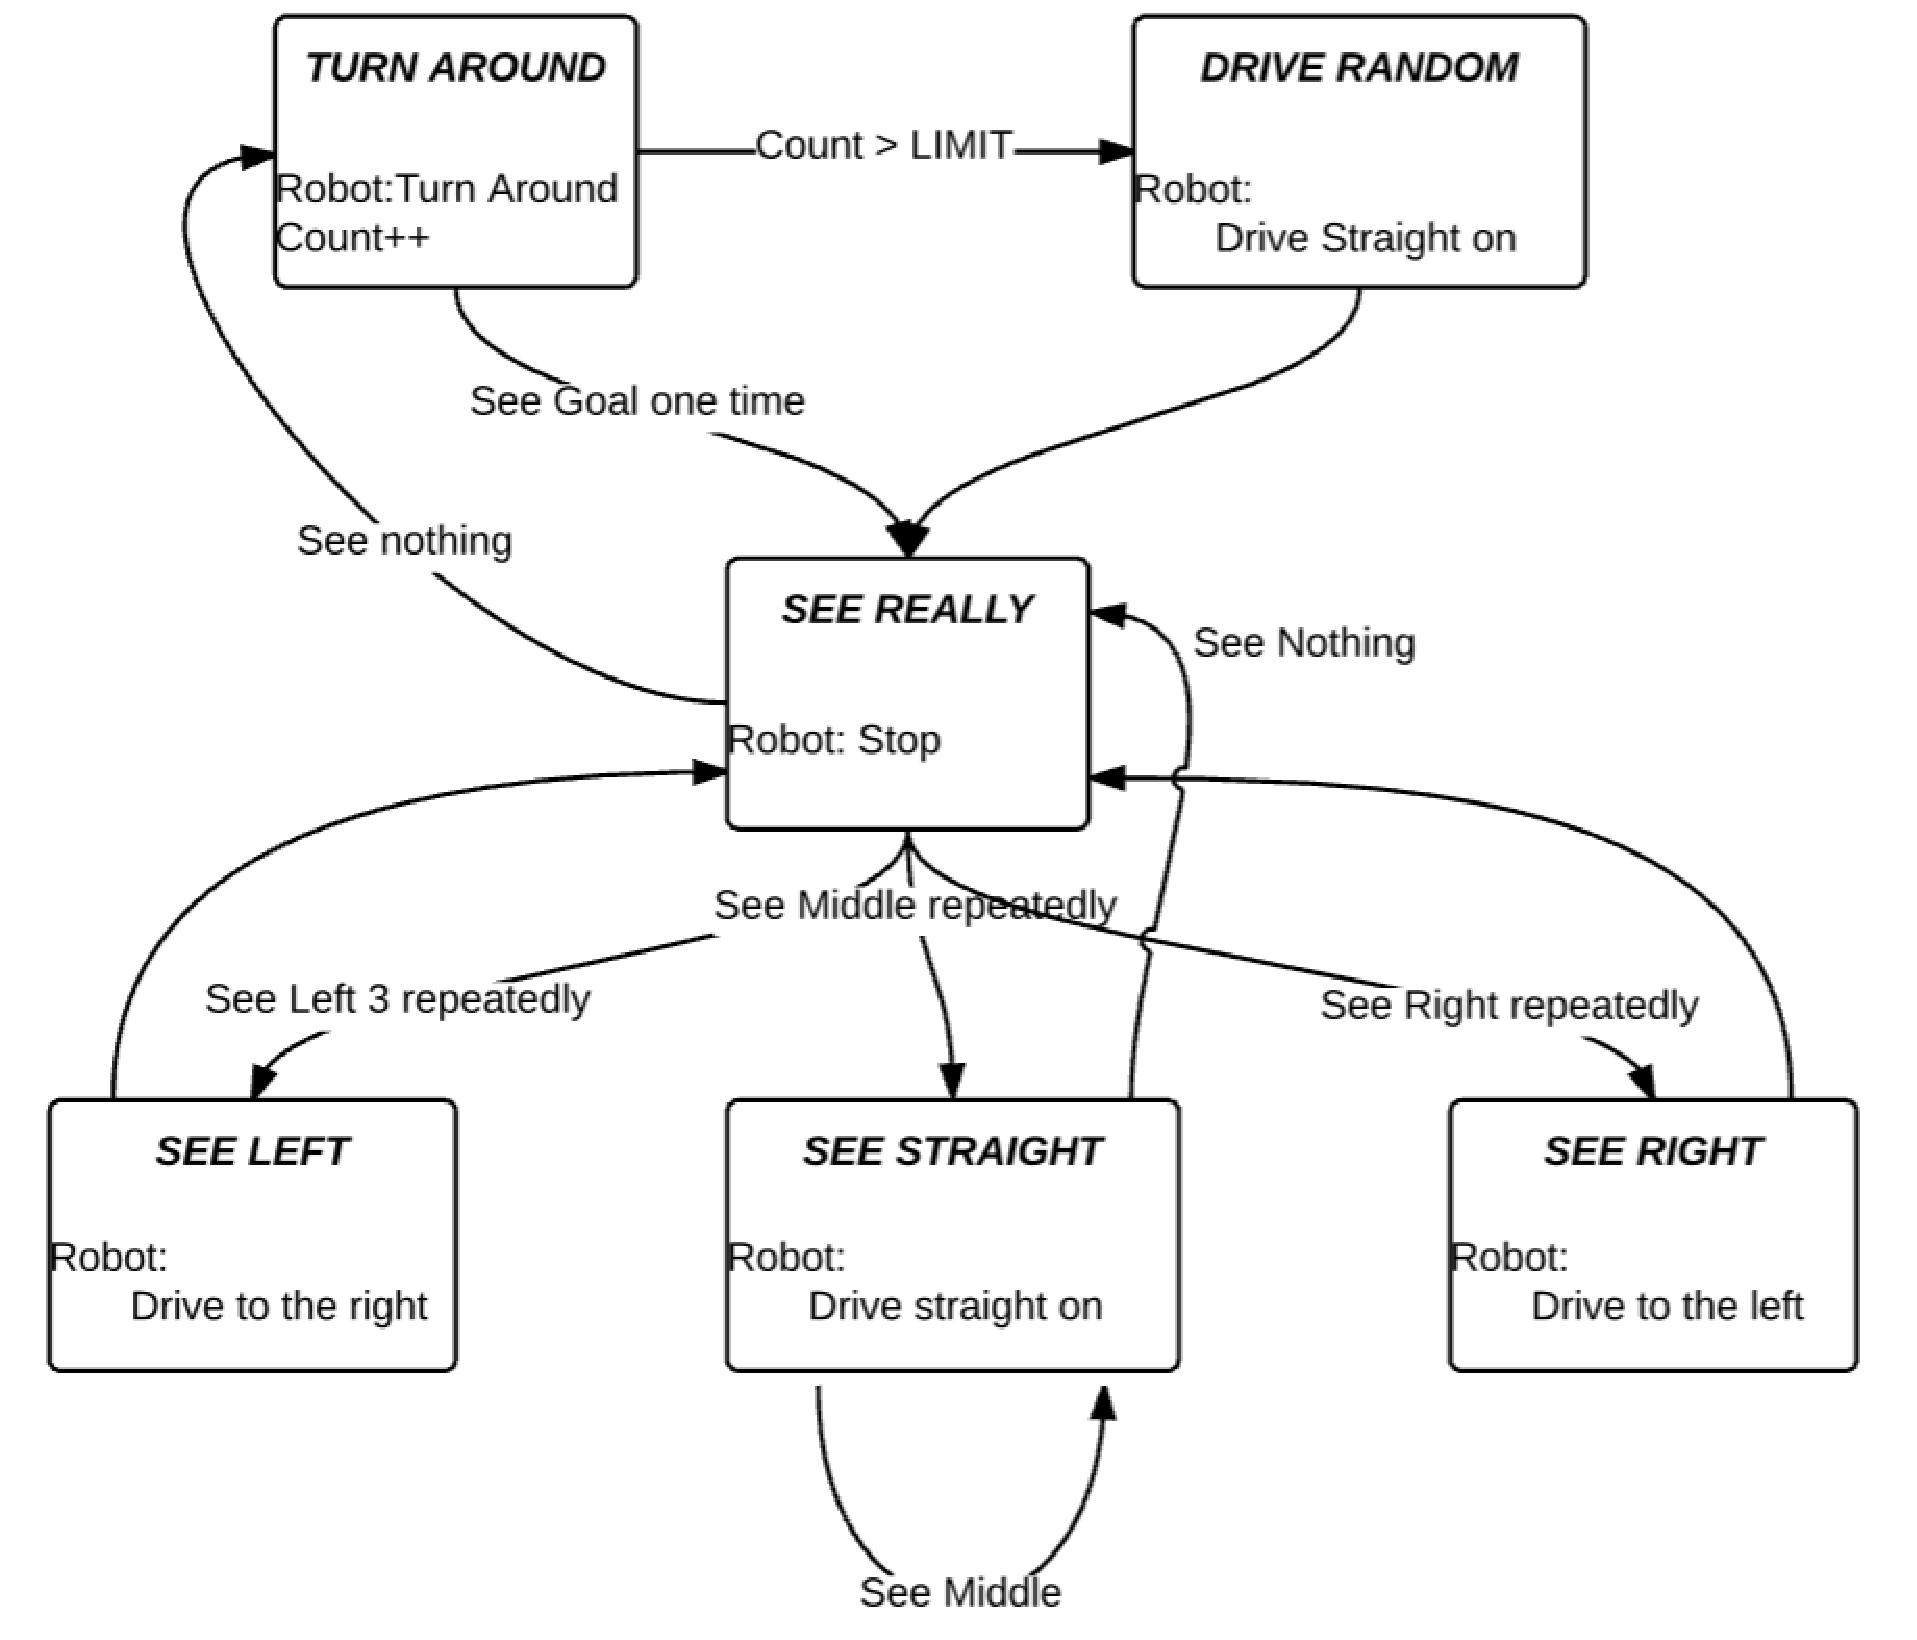
\includegraphics[width=\textwidth]{images/state_diagramm_findgoal.pdf}
	\caption{Zustandsdiagramm der Torfindung}
	\label{fig:state_findgoal}
\end{figure}

Diese Methode hier gut geeignet, da mit jedem Roboter Status dieselbe Routine aufgerufen wird. Mithilfe der Zustände lässt sich hier gut auf die unterschiedlichen Anforderungen reagieren. Auf den gleichen Status vom Roboter muss unterschiedlich reagiert werden, je nachdem in welchem Zustand sich der Roboter befindet. Der Code hierzu befindet sich in der Klasse \textit{EnergyManager} \cite{PROJEKT}\\
Der Nachteil bei dieser Implementierung ist natürlich die unsichere Verhaltensweise des Roboters, wenn er außerhalb der LED-Reichweite ist. Diese führt im Worst-Case zu einer kompletten Entladung des Akkus bis zur Bewegungsunfähigkeit, bevor die Station gefunden wurde. Da der Großteil des Spielfelds jedoch von den LEDs abgedeckt wird, ist dieser Fall unwahrscheinlich. Ein Vorteil dieser Methode im Gegensatz zu zum Beispiel einer Kamera basierten Positionsbestimmung ist die Unabhängigkeit des Spielfelds. Lediglich die LEDs müssen am Tor vorhanden sein, jedoch keine speziellen Konturen oder andere feste Muster, an denen der Roboter sich mithilfe der Kamera orientieren kann. Abgesehen davon ist die Torfindung mittels IR-LEDs vergleichsweise einfach zu realisieren.

\begin{figure}[!h]
	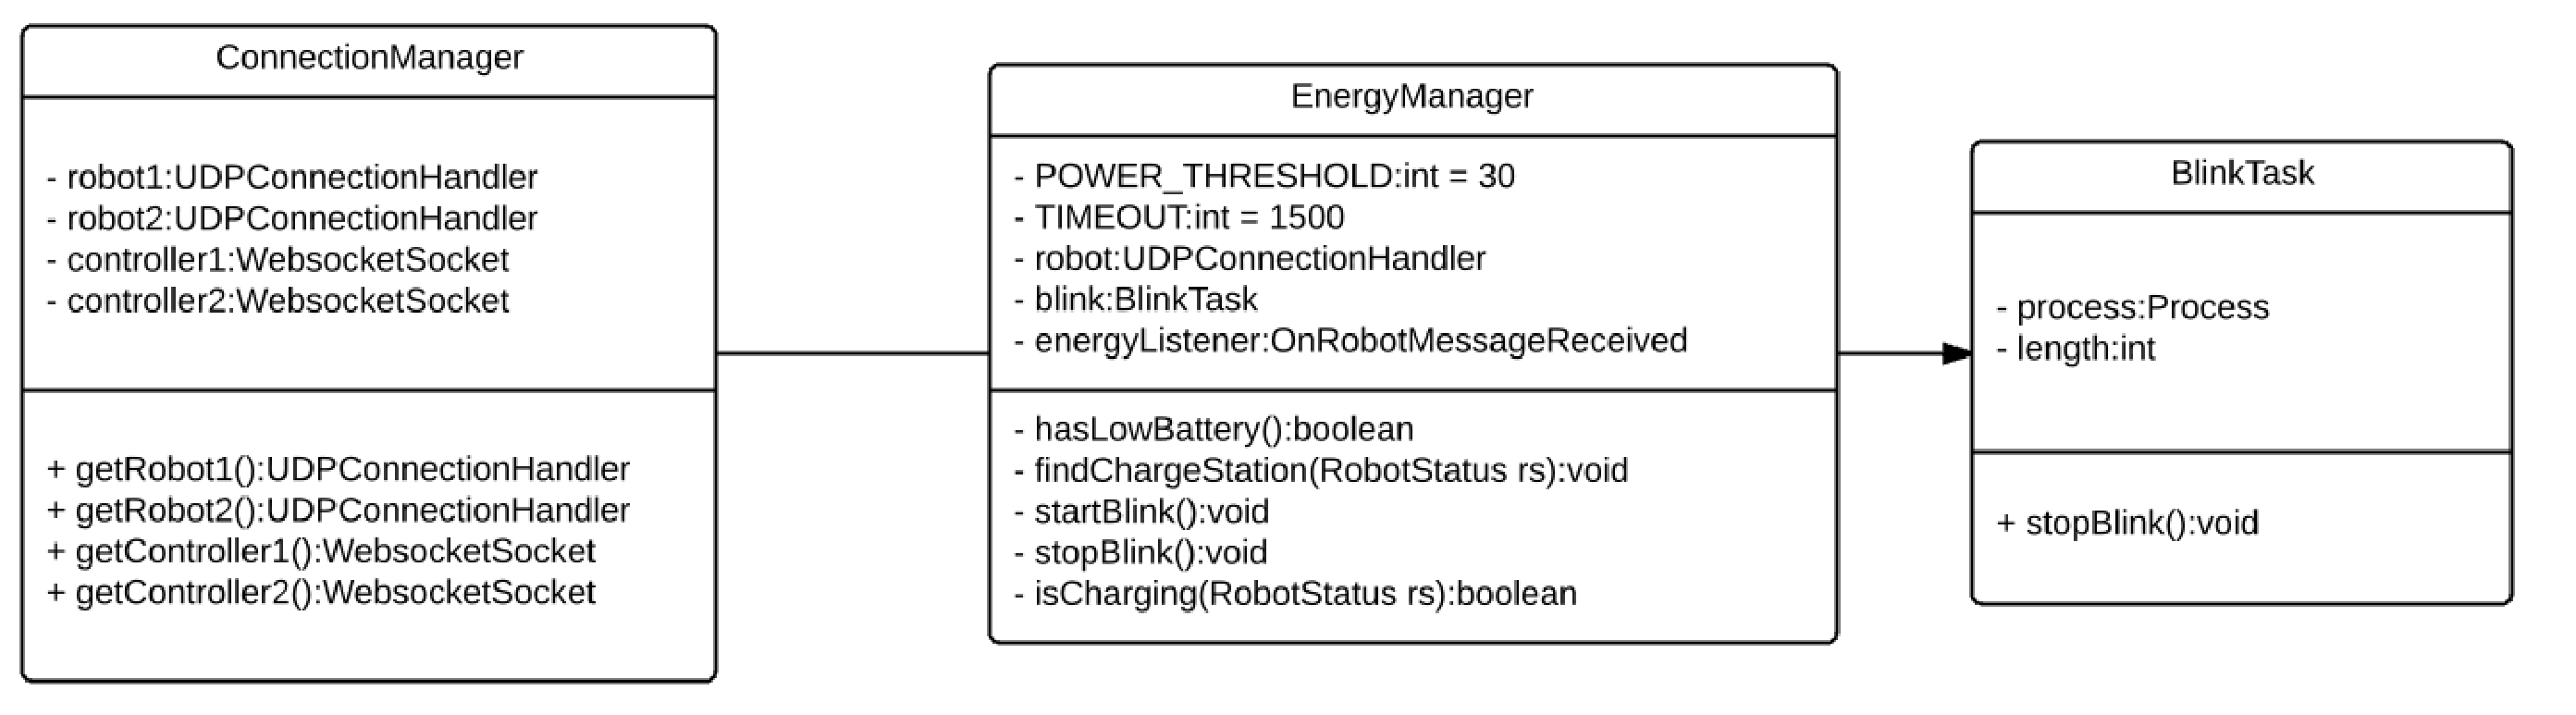
\includegraphics[width=\textwidth]{images/uml_energymanager.pdf}
	\caption{Klassendiagramm der Torfindung}
	\label{fig:uml_energymanager}
\end{figure}




\section{Webanwendung}
\label{sec:webanwendung_anwendung}

Die Webanwendung stellt eine Steuerungsvariante dar, die von überall aus genutzt werden kann, wo eine Tastatur und ein Browser vorhanden sind. Sie ist in Javascript implementiert und wird direkt von einem ebenfalls auf dem Server installierten Jetty-Webserver gehostet. Aufgerufen werden kann er über die IP-Adresse des Host-Systems unter Port 8080. Dabei funktioniert die Kommunikation genau wie bei der Android-Anwendung über einen WebSocket, der die gegebene Kommunikationsschnittstelle für die Controller auf dem Server nutzt. 
Die Oberfläche besteht lediglich aus einem Container für die Bilddaten. 
Über die gewohnte Pfeiltasten-Steuerung kann der Roboter gesteuert werden. Die gedrückten Tasten werden hierbei nur an den Server weitergegeben, erst dort werden sie verarbeitet (siehe Abschnitt \ref{sec:webanwendung_server}).

\section{Android-Anwendung}
Als mobile Anwendung für Endgeräte wurde Android ausgewählt, da diese Plattform einige Vorteile bietet. Im Gegensatz zu anderen mobilen Betriebssystemen ist es für Android möglich, ohne Lizenzen oder andere Absprachen zu treffen, Anwendungen zu entwickeln. Außerdem kann hiermit auch in Java entwickelt werden und der Zugriff auf die Sensorik des Geräts ist bereits sehr gut vorbereitet. 
Die Anwendung vereint mehrere Steuerarten, die sich in ihrem Abstraktionsgrad unterscheiden. Diese werden in den folgenden Abschnitten beschrieben.

Die Software ist wie in Anhang \ref{fig:android_uml} dargestellt konzipiert. Den Mittelpunkt der Android-Anwendung stellt die abstrakte Klasse \textit{ControlActivity} dar. Jede Steueractivity erbt von dieser Klasse. Damit ist es möglich, das gesamte gemeinsame Verhalten der Steuerungen (Anzeigen des Spielstands und der Bilddaten, Reaktion auf Verbindungsabbrüche etc..) in einer Zentrale zu implementieren. Jede Subklasse implementiert hierbei lediglich die Art, wie Befehle akquiriert werden. 

\begin{figure}[!h]
	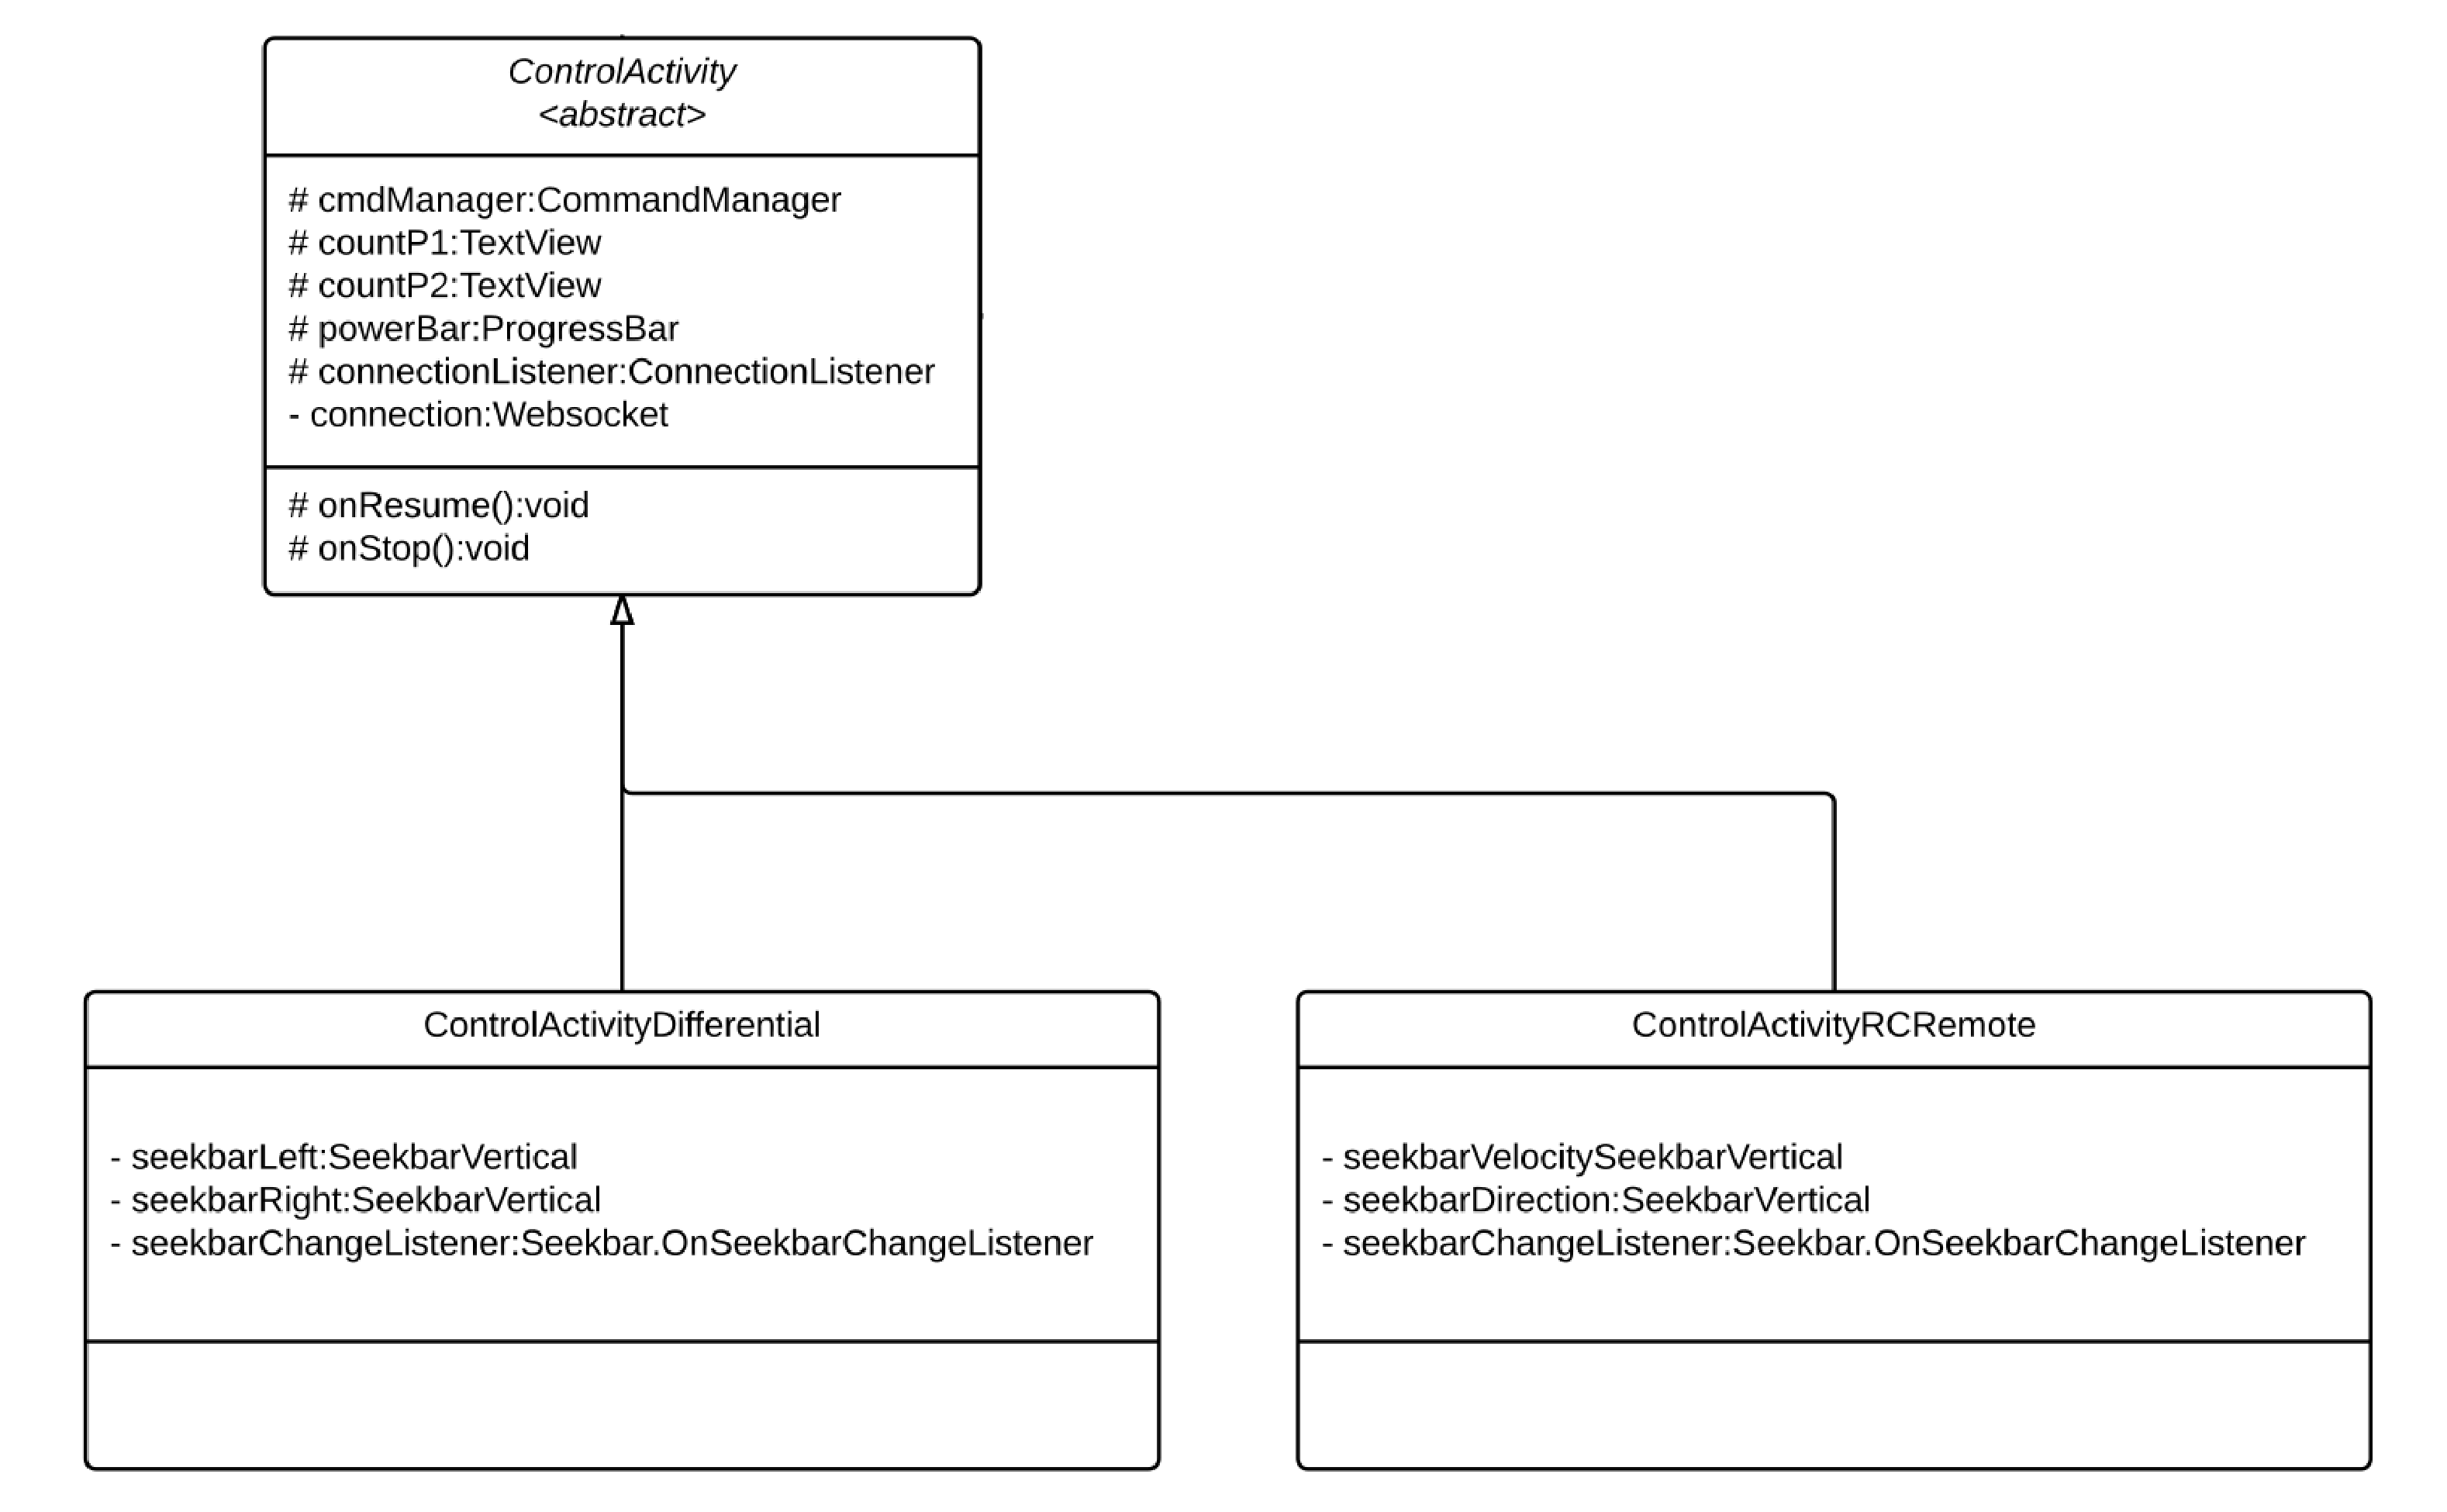
\includegraphics[width=\textwidth]{images/uml_controlactivity_android.pdf}
	\caption{Klassendiagramm ControlActivities}
	\label{fig:uml_controlactivity_android}
\end{figure}

Der Schussauslöser wird in jedem Fall über die Beschleunigungssensorik des Geräts implementiert. Hierbei wird die auf das Gerät wirkende Beschleunigung gemessen und ab einem gewissen Grenzlevel der Schuss herbei geführt, was darin resultiert, dass der Schuss über ein kurzes Schütteln des Geräts erreicht wird.
Wie auch in der Serverimplementierung gibt es hier eine Klasse, die aktuelle Befehlsänderungen puffert und mit einer Frequenz von 10Hz über den Websocket an den Server sendet.
Die Klassen \textit{Websocket}, \textit{CommandManager} und \textit{ControlActivity} bilden im Klassendiagramm eine Art Regelkreis der wie folgt interpretiert werden kann. In der \textit{ControlActivity} wird der Befehl akquiriert, im \textit{CommandManager} dann in einen Befehl umgewandelt und über den Websocket versendet. Über den \textit{Websocket} werden anschließend die Bilddaten vom Server empfangen und an die \textit{ControlActivity} weitergegeben, worauf der Benutzer reagieren kann und seine Steuerbefehle dementsprechend anpasst.
 

\subsection{Differential Steuerung}
\label{sec:differentialsteuerung}

Diese Steuerung ist die am wenigsten abstrahierte Steuerung. Es gibt zwei vertikal ausgerichtete Slider, die jeweils für den linken oder den rechten Motor stehen und einen Wertebereich von -100 - +100 abdecken. Bewegt man den Slider nach oben, beschleunigt der Roboter vorwärts, nach unten dementsprechend rückwärts. Wie oben bereits erwähnt, wird der Schuss über die Sensorik des Geräts ausgelöst. Mit dieser Steuerung sind die genauesten Bewegungen möglich, da man das volle Potenzial ausschöpfen kann. Im Gegensatz zu den anderen Steuerungen werden keine Befehle limitiert. Jedoch wird die Steuerung dadurch sehr schwierig und für Anfänger nur schwer benutzbar.

\begin{figure}[h!]
	\centering
	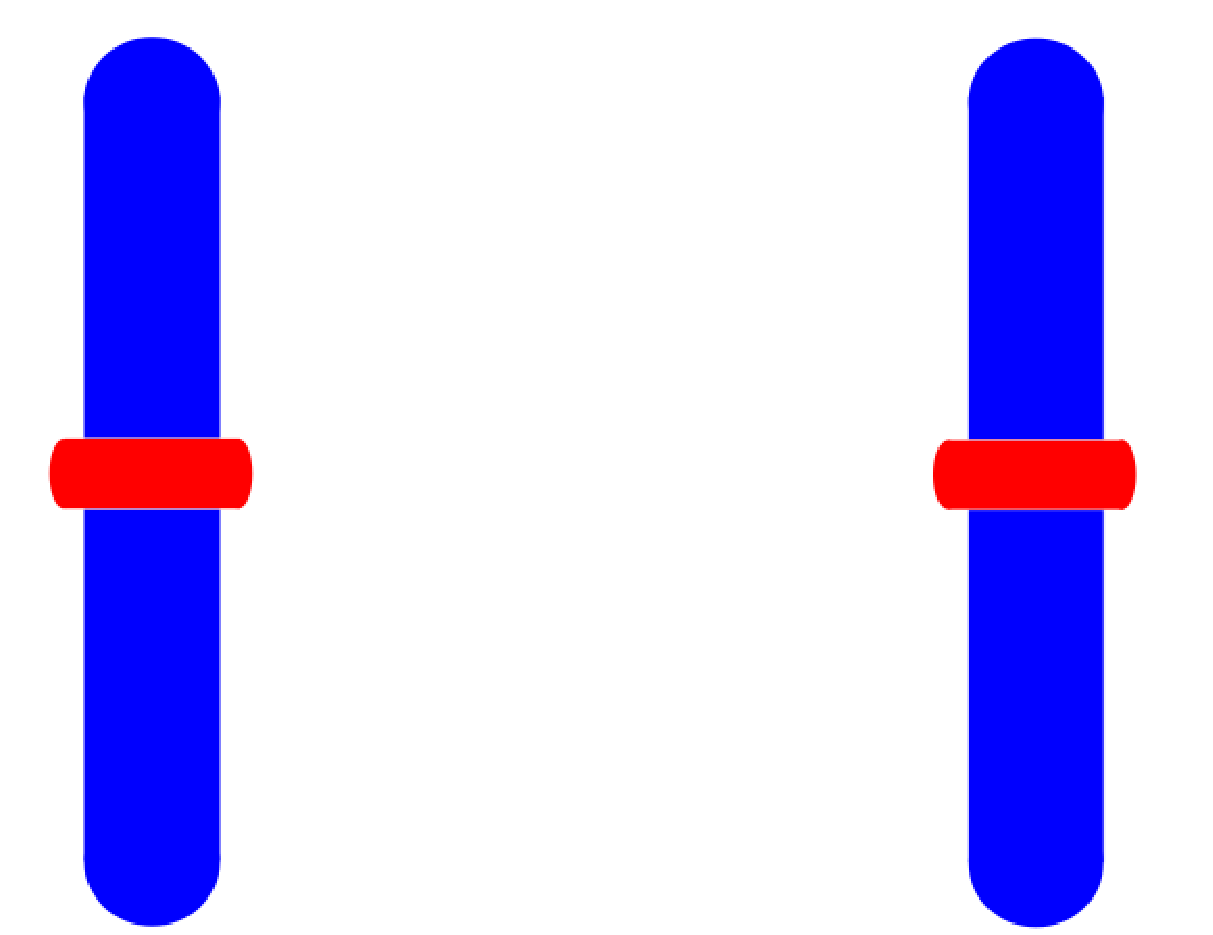
\includegraphics[height=.25\textheight]{images/android_diff.pdf}
	\caption{Schematische Darstellung der Differential Steuerung}
	\label{fig:android_diff}
\end{figure}

\subsection{RC-Remote Steuerung}

Ähnlich wie in der Differential Steuerung kommen auch hier Slider zum Einsatz. Der vertikale Slider steht hierbei für die Beschleunigung des Roboters und der horizontale für die Winkel, den der Roboter einschlägt, ähnlich wie man es von einer Fernbedienung von ferngesteuerten Spielzeugautos kennt. Auch hier wird der Schuss über die Sensoren ausgelöst. Der Beschleunigungsregler hat einen Wertebereich von -100 bis +100. Dadurch bildet er genau die Leistung ab, die jeder Motor annehmen soll (solange keine Richtung angegeben wird). Der Richtungsregler hat einen Wertebereich von -50 - +50, wobei der tatsächliche Intervall keine Rolle spielt, da der Winkel, der eingeschlagen wird relativ zum Gesamtintervall berechnet wird (siehe \ref{sec:rcremote_server}). Ein großer Vorteil gegenüber den Differential Steuerung ist die leichtere Bedienbarkeit. Da nicht mehr jeder Motor separat angesteuert werden muss ist es zum Beispiel sehr einfach, den Roboter nur gerade aus zu steuern. Jedoch ist der maximale Winkel den man einschlagen kann begrenzt und auch die Möglichkeit sich auf der Stelle zu drehen fällt bei dieser Steuerung weg. Die Umsetzung erfolgt in der Serverlogik und ist in Abschnitt \ref{sec:rcremote_server} beschrieben.


\begin{figure}[h!]
	\centering
	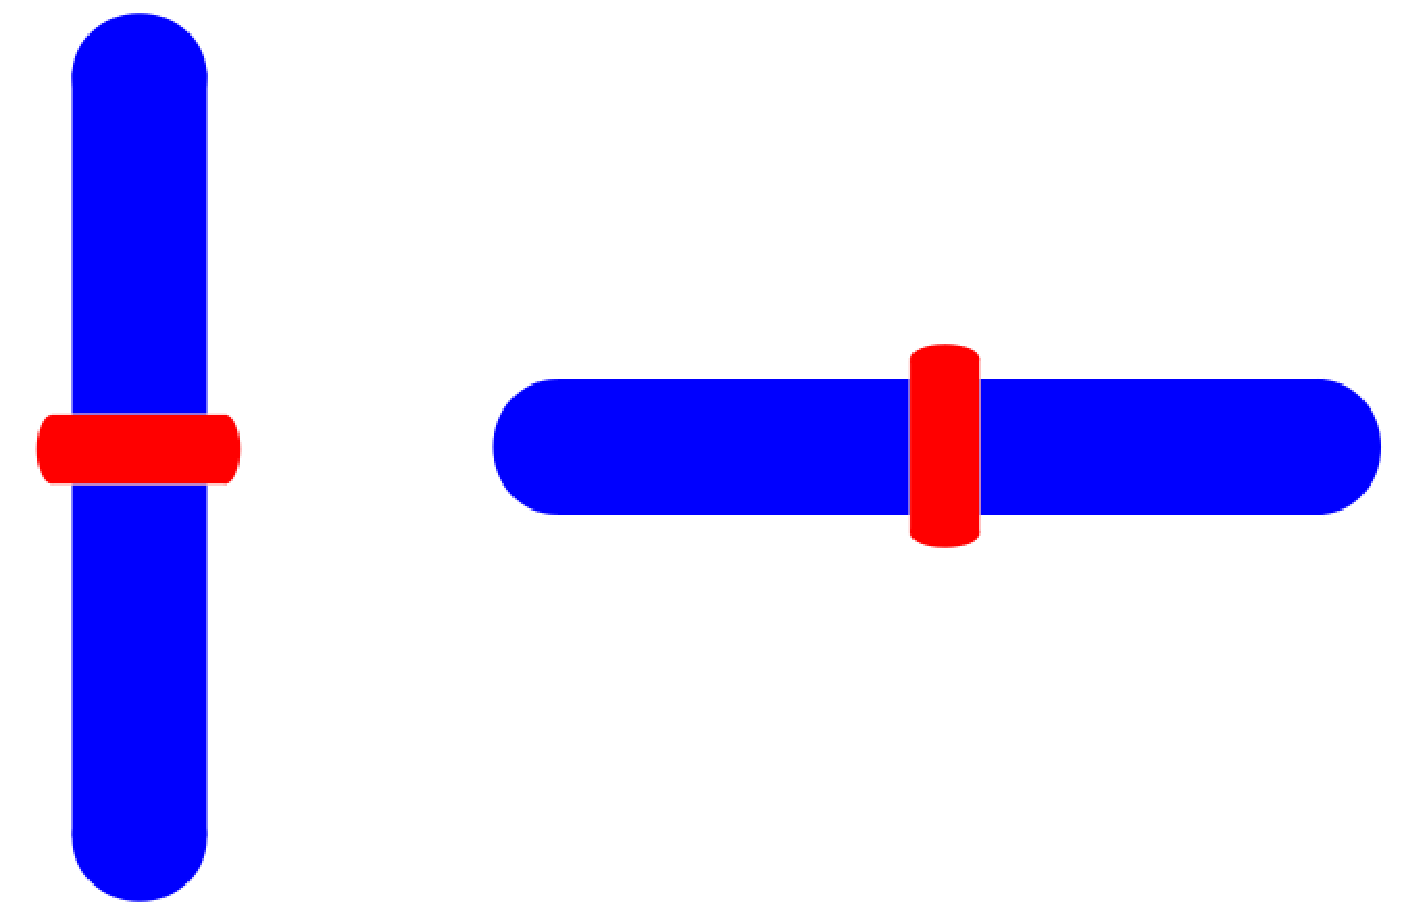
\includegraphics[height=.25\textheight]{images/android_rcremote.pdf}
	\caption{Schematische Darstellung der RCRemote Steuerung}
	\label{fig:android_rcremote}
\end{figure}



\section{RobotSimulator}
Einige Komponenten im Code des Servers benötigen gewisse Informationen vom Roboter, wie zum Beispiel die Bildübertragung. Da die Roboter gleichzeitig zur Steuerung entwickelt wurden und deswegen nicht rund um die Uhr zur Verfügung standen war es hilfreich einen Simulator zu entwickeln, der Befehle im exakt selben Format versendet. So wurde die gesamte Roboter-Server Kommunikation simuliert. Hierzu wurde ein Paket mit festen Werten erstellt, das genau wie der Roboter auch, alle 100ms per UDP an den Server gesendet wird.\\
Um die Bilddatenpufferung des Servers testen zu können, wurden zwei Beispielbilder von der Festplatte in ein großes Byte-Array geladen. So war es möglich die Eigenschaft des Roboters zu simulieren, Bilddaten ohne Trennung, also keine separierten Bilder zu senden (vgl. Listing \ref{code:robot_sim}). \\

\begin{lstlisting}[captionpos = b, caption=Quellcode des RobotSimulators zum Testen der Kameraübertragung, label = code:robot_sim]
puffer = new byte[puffer1.length + puffer2.length];
System.arraycopy(puffer1, 0, puffer, 0, puffer1.length);
System.arraycopy(puffer2, 0, puffer, puffer1.length, puffer2.length);
				.
				.
				.
private static void fillBuffer() {
	// puffer is byte[] with two pictures concatenated
	// data is the packet to send
	for (int i = 0; i < 1400; i++) {
		data[i + 12] = puffer[pointer];
		pointer++;
		if (pointer == puffer.length) {
			pointer = 0;
		}
	}
}
\end{lstlisting}

Ein weiterer Vorteil dieser Methode, abgesehen von der ständigen Verfügbarkeit, lag an der klaren Abtrennung von auftretenden Problemen. Wurde der Simulator erst einmal richtig konfiguriert, war die Schnittstelle für beide Seiten definiert. Funktionierte hinterher im Test etwas bei der Kommunikation nicht, konnten lediglich die Pakete des Simulators mit denen des Roboters verglichen werden. Unterschieden sie sich, war der Fehler auf der Roboter Seite.